%%%%%%%%%%%%%%%%%%%%%%%%%%%%%%%%%%%%%%%%%
% FRI NLP Final Report
%%%%%%%%%%%%%%%%%%%%%%%%%%%%%%%%%%%%%%%%%

\documentclass[fleqn,moreauthors,10pt]{ds_report}
\usepackage[english]{babel}
\usepackage{hyperref}
\usepackage{graphicx}
\usepackage{booktabs}
\usepackage{array}
\usepackage{tabularx}
\graphicspath{{fig/}{figures/}}

\JournalInfo{FRI Natural Language Processing Course 2026}
\Archive{Final project report}

\PaperTitle{
\begin{center}
Final Report\\[0.3em]
Domain-Specific Fitness NLP Assistant Using Retrieval-Augmented Generation
\end{center}
}
\Authors{Domen Pahole, Luka Rizman, Nina Trivi\'c}

\affiliation{\textit{Advisors: Ale\v{s} \v{Z}agar}}

\Keywords{Natural Language Processing, Retrieval-Augmented Generation, Fitness Assistant, Semantic Retrieval, Large Language Models}
\newcommand{\keywordname}{Keywords}

\Abstract{
We present a domain-specific fitness assistant built around Retrieval-Augmented Generation (RAG). The system combines a sentence-transformer retriever, a Qdrant vector database, and the Llama 3.2 1B model served through Ollama. Our main goal is not to maximize raw language fluency, but to improve grounding to a fixed exercise dataset and reduce unsupported recommendations. On an 11-query retrieval benchmark, the system reaches Hit@1 = 0.636, Hit@3 = 0.909, Hit@5 = 0.909, Precision@5 = 0.582, and MRR = 0.742. Qualitative comparison against the same 1B model without retrieval shows that RAG produces more dataset-aligned answers when retrieval succeeds, but also inherits retrieval failures. The main take-away is that, for this project, retrieval quality is the dominant bottleneck and the most promising direction for future improvement.
}

\begin{document}
\flushbottom
\maketitle
\thispagestyle{empty}
\fancyhf{}
\fancyhead[R]{\small\sffamily\bfseries \thepage/\pageref{LastPage}}
\renewcommand{\headrulewidth}{0pt}
\setlength{\headheight}{14pt}

\section*{1 Introduction}

General-purpose LLMs are often fluent, but they are not reliable domain experts when answers depend on a specific local knowledge base. Our project addresses this problem in the fitness domain. We build a conversational assistant that answers questions about exercises, equipment, muscle groups, and training suggestions using a structured exercise dataset rather than relying only on the model's parametric knowledge.

The project follows the course topic of domain-specific AI assistants. We define a narrow use case, prepare a domain knowledge base, implement retrieval and generation components, and evaluate both retrieval quality and end-to-end answer behavior. The final system is designed to be easy to rerun locally or on HPC, with all dependencies and scripts available in the repository.

\section*{2 Data and System}

\textbf{Dataset.} We use the MegaGym exercise dataset, which contains 2,918 exercise entries. Each entry includes a title, description, exercise type, target body part, equipment, difficulty level, and optional rating fields. The dataset is public and linked in the repository instructions, so it is not duplicated in version control.

\textbf{Knowledge representation.} Each exercise is converted into a textual record containing the title, description, type, body part, equipment, difficulty level, and rating metadata. These records are embedded and stored in Qdrant.

\textbf{Retriever.} We use the Sentence Transformers model all-MiniLM-L6-v2. Retrieval uses cosine similarity in Qdrant with default depth top-$k=5$.

\textbf{Generator.} For answer generation we use Llama 3.2 1B through Ollama. This choice follows the course constraint to use a small model that can also run on HPC. The same model is used in both baseline and RAG settings, so the comparison isolates retrieval effects rather than model size.

\textbf{Prompting.} In the RAG setting, the prompt instructs the model to use only retrieved exercise entries, prefer matches by body part, equipment, and difficulty, remove duplicates, and explicitly state when the dataset is insufficient. The baseline prompt receives only the user question.

\textbf{Implementation details.} The repository contains a Streamlit interface, indexing script, retrieval evaluation script, baseline-vs-RAG comparison script, and a unified evaluation runner. The system can run locally with Docker-based Qdrant or on Arnes HPC with local Qdrant storage and Ollama on a GPU node.

\begin{table}[h]
\centering
\caption{Algorithm settings used for all reported results. The table is self-contained: it specifies the model choices, retrieval setup, and operational hyperparameters needed to rerun the same pipeline.}
\label{tab:algorithm-settings}
\small
\begin{tabularx}{\columnwidth}{@{}>{\raggedright\arraybackslash}p{0.32\columnwidth} >{\raggedright\arraybackslash}X@{}}
\toprule
Component & Final setting \\
\midrule
Retriever encoder & Sentence Transformers all-MiniLM-L6-v2 (384-dimensional embeddings) \\
Vector database and search & Qdrant collection \texttt{megagym\_exercises}, cosine similarity \\
Retrieval depth & Top-$k=5$ for app responses and evaluation scripts \\
Main improvement in prompting & Use only retrieved entries, prioritize body part/equipment/difficulty matches, remove near-duplicates, and explicitly state when context is insufficient \\
Generator & \texttt{llama3.2:1b} via Ollama (same model in baseline and RAG) \\
Indexing/runtime hyperparameters & Embedding batch size 64, Qdrant upsert chunk size 512, Ollama request timeout 180\,s \\
\bottomrule
\end{tabularx}
\end{table}

\begin{figure}[h]
\centering
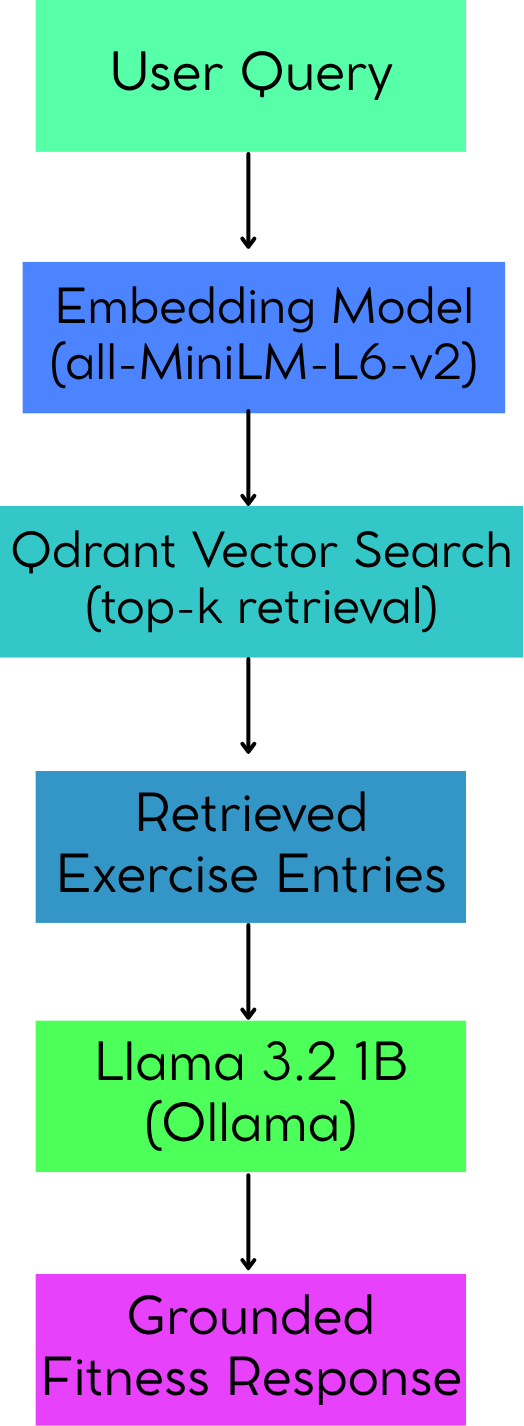
\includegraphics[width=0.58\columnwidth,height=0.45\textheight,keepaspectratio]{rag_pipeline.png}
\caption{RAG pipeline used in the fitness assistant: user query, retrieval from Qdrant, and grounded generation with Llama 3.2 1B.}
\label{fig:rag-pipeline}
\end{figure}

\section*{3 Evaluation Setup}

We evaluate the system in two complementary ways.

\textbf{Retrieval evaluation.} We created a small benchmark of 11 natural-language fitness queries with manually specified expectations. Each query defines relevant properties such as body part, equipment, difficulty level, and keywords. Retrieved items are marked relevant if they satisfy these constraints. We report Hit@1, Hit@3, Hit@5, Precision@5, and Mean Reciprocal Rank (MRR).

\textbf{End-to-end comparison.} We compare baseline generation and RAG generation on five representative questions. For each question, we manually select the better answer based on constraint alignment (body part, equipment, difficulty) and dataset grounding. This gives a compact per-query winner table while keeping the same model fixed in both settings.

\section*{4 Results}

Table~\ref{tab:main-results} summarizes the main quantitative results of the retrieval component.

\begin{table}[h]
\centering
\caption{Retrieval evaluation on 11 manually specified fitness queries. Higher is better for all metrics. The table is self-contained: Hit@$k$ measures whether at least one relevant exercise appears in the top $k$ retrieved items, Precision@5 measures the fraction of relevant items among the top five, and MRR measures how early the first relevant result appears.}
\label{tab:main-results}
\begin{tabular}{lr}
\toprule
Metric & Value \\
\midrule
Queries & 11 \\
Hit@1 & 0.636 \\
\textbf{Hit@3} & \textbf{0.909} \\
\textbf{Hit@5} & \textbf{0.909} \\
Precision@5 & 0.582 \\
MRR & 0.742 \\
\bottomrule
\end{tabular}
\end{table}

The results show that retrieval is already strong enough to support a useful RAG pipeline. In 10 out of 11 queries, at least one relevant exercise appears in the top five retrieved items. However, the lower Hit@1 score shows that the first retrieved result is still often suboptimal. This matters because the generator is sensitive to noisy or weak context.

Table~\ref{tab:e2e-comparison} summarizes the end-to-end comparison in one consolidated format so the reader can compare systems query-by-query.

\begin{table}[h]
\centering
\caption{Consolidated baseline-vs-RAG comparison on five representative questions using the same Llama 3.2 1B model. ``Better'' is decided by manual judgment of alignment with query constraints and grounding in retrieved MegaGym entries. The last row reports total wins; the best total is bolded.}
\label{tab:e2e-comparison}
\small
\begin{tabularx}{\columnwidth}{@{}>{\raggedright\arraybackslash}p{0.29\columnwidth} >{\raggedright\arraybackslash}p{0.17\columnwidth} >{\raggedright\arraybackslash}X@{}}
\toprule
Query & Better & Evidence \\
\midrule
Triceps with cable & \textbf{RAG} & Uses cable-triceps exercises directly matching retrieved dataset entries, while baseline remains generic. \\
Beginner bodyweight legs & \textbf{Baseline} & Retrieved set is partially mismatched (plyometrics and off-target items), so RAG inherits retrieval errors. \\
Back with pull-up bar & \textbf{Baseline} & RAG includes off-target suggestions (e.g., squat), while baseline stays closer to the requested equipment. \\
Biceps with barbell & \textbf{RAG} & More grounded barbell naming from retrieved entries; baseline includes broader generic advice. \\
Abs with exercise ball & \textbf{RAG} & Better dataset-grounded naming of exercise-ball abdominal variants. \\
\midrule
Total wins (5 queries) & Baseline 2 / \textbf{RAG 3} & Best overall end-to-end score in this project is RAG. \\
\bottomrule
\end{tabularx}
\end{table}

\noindent Related prior work in fitness recommendation \cite{Yang2023} is contextually relevant but not directly comparable numerically here because it targets a different setup and does not report MegaGym retrieval metrics such as Hit@$k$ or MRR.

\section*{5 Analysis of Successes and Failures}

Our qualitative analysis shows that Retrieval-Augmented Generation improves answer grounding when retrieval quality is sufficiently strong, but also exposes weaknesses when retrieval results are noisy or incomplete.

\subsection*{5.1 Successful Retrieval Example}

The clearest success case is the query:

\begin{quote}
\emph{``Can you recommend some triceps exercises that use a cable machine?''}
\end{quote}

In the baseline setting, the model produces plausible but generic cable-triceps suggestions without strong alignment to the dataset. In contrast, the RAG version retrieves exercises such as \emph{Cable Straight-Bar Push-Down} and \emph{Triceps Overhead Extension with Rope}, which closely match the intended muscle group and equipment constraints.

This example demonstrates the main advantage of RAG in our project: the same small language model becomes substantially more domain-grounded when retrieval provides relevant context.

\subsection*{5.2 Retrieval Failure Example}

One representative failure case is the query:

\begin{quote}
\emph{``Which bodyweight leg exercises would you suggest for a beginner?''}
\end{quote}

Here, retrieval quality degrades noticeably. Some returned exercises are only partially related to beginner leg training, while others contain unclear naming or inconsistent metadata. For example, one retrieved result was \emph{``30 Flat Bench Leg Raise''}, which is ambiguously named and does not clearly correspond to the intended query constraints.

Additionally, some retrieved exercises target unrelated muscle groups such as abdominals rather than legs. Because the generator depends directly on retrieved context, the final RAG response inherits these retrieval errors and becomes less useful than the baseline answer.

This example highlights an important limitation of RAG systems: retrieval does not automatically improve answer quality. The generation stage is only as reliable as the retrieved context it receives.

\subsection*{5.3 Incomplete Retrieval and Metadata Noise}

We also observe partial failures caused by incomplete retrieval results, noisy metadata, and near-duplicate entries in the dataset.

For example, for the query:

\begin{quote}
\emph{``Back exercises with dumbbells''}
\end{quote}

the system generated only three meaningful exercise suggestions before producing a \emph{``No data available''} output for the fourth retrieved item. This indicates that retrieval sometimes fails to provide sufficiently complete or relevant context for stable answer generation.

Additional problems originate from inconsistent dataset formatting. Some exercise descriptions are repeated, some titles are near-duplicates, and certain metadata fields are missing or weakly standardized. These issues reduce retrieval precision and make the prompt context noisier than intended.

Overall, our analysis suggests that retrieval quality is the dominant bottleneck of the current system. When retrieval is strong, RAG substantially improves grounding and specificity. When retrieval is weak or noisy, the final answer quality degrades quickly.

\section*{6 Discussion}

The main conclusion is that retrieval quality dominates final answer quality in this project. Our main improvement over baseline is the grounding-constrained RAG prompt: the model is forced to use retrieved entries, prioritize body part/equipment/difficulty matches, remove duplicates, and admit insufficient evidence. This improves specificity when retrieval is good and makes failure cases easier to diagnose when retrieval is noisy.

This finding is practically useful for future work. The most promising improvements are not larger models, but better retrieval and cleaner data. In particular, the next steps should include:

\begin{itemize}
\item metadata-aware filtering by body part, equipment, and difficulty,
\item dataset cleaning and deduplication,
\item expansion of the evaluation benchmark beyond 11 retrieval queries,
\item more systematic human evaluation of final answers.
\end{itemize}

Our work is also consistent with the general motivation of RAG systems \cite{Lewis2020}: retrieval can inject task-specific knowledge into a fixed generator. In the fitness domain, related work has also explored exercise recommendation systems that combine structured information and NLP components \cite{Yang2023}. Our contribution is smaller in scale, but it demonstrates the same core principle in a reproducible course project setting.

\section*{7 Reproducibility and Final Take-Away}

The repository is structured so that another student can rerun the project with minimal setup. Dependencies are pinned in \path{requirements.txt}; local setup and HPC setup are documented in \path{LOCAL_SETUP.md} and \path{peer-review.md}. The MegaGym dataset is linked (not versioned), indexing and evaluation scripts are included, and results are written to \path{report/results/}. This satisfies the requirement that reviewers can understand and rerun the full pipeline.

\textbf{Take-away message.} With the same small 1B language model, RAG improves domain grounding by forcing answers to use retrieved MegaGym exercise entries. The main limitation is not the generator itself, but retrieval quality: when retrieval is strong, answers become more specific and trustworthy; when retrieval is weak, the whole system fails with it.

\bibliographystyle{unsrt}
\bibliography{report}

\end{document}